\chapter{Payload Deployment}

During the boost, coast, and the majority of the launch vehicle's flight, the payload will remain idle and securely fixed in the payload bay. This chapter will detail the means of securement and deployment of the payload, as well as a trade-off between the various means that have been consider to arrive at the leading design.

This chapter will be structured as follows: Sec.~\ref{PL:Deployment:Requirements} details the requirements the payload is to satisfy given the overall mission and top-level requirements, followed by a trade-off study regarding the means of securement in Sec.~\ref{PL:Deployment:Securement}, as well as the possible deployment modes in Sec.~\ref{PL:Deployment:Deployment}. Finally, the leading design is presented in Sec.~\ref{PL:Deployment:LeadingDesign} in reference to the foregoing trade-off studies.


\section{Requirements}\label{PL:Deployment:Requirements}

This section details the various requirements to which the payload deployment scheme must abide. Specifically, two forms of requirements are identified: top-level requirements and team-derived requirements. The first are requirements either imposed by the competition, or legislation that is in effect at the time of launch and operations. The second form of requirements pertain to what the team perceives to be of importance in assuring mission success and robustness.

\subsection{Top-level requirements}

The top-level requirements for the payload deployment are outlined in Secs. 4.3--4 of \citep{MSFC2019}, reading as follows:

\begin{enumerate}[noitemsep, label=4.\arabic*.]
	\setcounter{enumi}{3}
	\item Lunar Ice Sample Recovery Mission Requirements
	\begin{enumerate}[noitemsep, label=4.3.\arabic*.]
		\setcounter{enumi}{5}
		\item Teams must abide by all \gls{faa} and \gls{nar} rules and regulations.
		\item Black Powder and/or similar energetics are only permitted for deployment of in-flight recovery systems. Any ground deployments must utilize mechanical systems.
		\item Any part of the payload or vehicle that is designed to be deployed, whether on the ground or in the air, must be fully retained until it is deployed as designed.
		\begin{enumerate}[noitemsep, label=4.3.7.\arabic*.]
			\item A mechanical retention system will be designed to prohibit premature deployment.
			\item The retention system will be robust enough to successfully endure flight forces experienced during both typical and atypical flights.
			\item The designed system will be fail-safe.
			\item Exclusive use of shear pins will not meet this requirement.
		\end{enumerate}
	\end{enumerate}
	\item Special Requirements for UAVs and Jettisoned Payloads
	\begin{enumerate}[noitemsep, label=4.4.\arabic*.]
		\item Any experiment element that is jettisoned during the recovery phase will receive real-time \gls{rso} permission prior to initiating the jettison event.
		\item \gls{uav} payloads, if designed to be deployed during descent, will be tethered to the vehicle with a remotely controlled release mechanism until the \gls{rso} has given permission to release the UAV.
		\item Teams flying \acrshortpl{uav} will abide by all applicable \gls{faa} regulations, including the \gls{faa}'s Special Rule for Model Aircraft (Public Law 112-95 Section 336; see \url{https://www.faa.gov/uas/faqs}).
		\item Any \gls{uav} weighing more than .55 lbs. will be registered with the \gls{faa} and the registration number marked on the vehicle.
	\end{enumerate}
\end{enumerate}

In addition, by \gls{faa} regulations \citep{FederalAviationAdministration2018}, the \gls{uav} may only be operated below \SI{400}{\feet} in \gls{los}\footnote{FAA Reauthorization Act of 2018 \S 346(b.2.C), 49 U.S.C. \S 44806}. From the FAA Reauthorization Act of 2018, the following pertinent regulations may be found. The \gls{uav} must have a gross weight under \SI{4.4}{\poundm}, and must be operated:

\begin{enumerate}[noitemsep, label=(\roman*)]
	\item within or beyond visual \gls{los} of the operator;
	\item less than \SI{400}{\feet} above ground;
	\item during daylight conditions;
	\item within Class G airspace; and
	\item outside of 5 statute miles from any airport, heliport, seaplane base, spaceport, or other location with aviation activities.
\end{enumerate}

As a supplement to these regulations, an aeronautical chart of the surroundings of the launch site (Bragg Farms, Hazel Green, AL) is given in Fig.~\ref{fig:PL:Deployment:VFRchart}.

\begin{figure}[H]
	\centering
	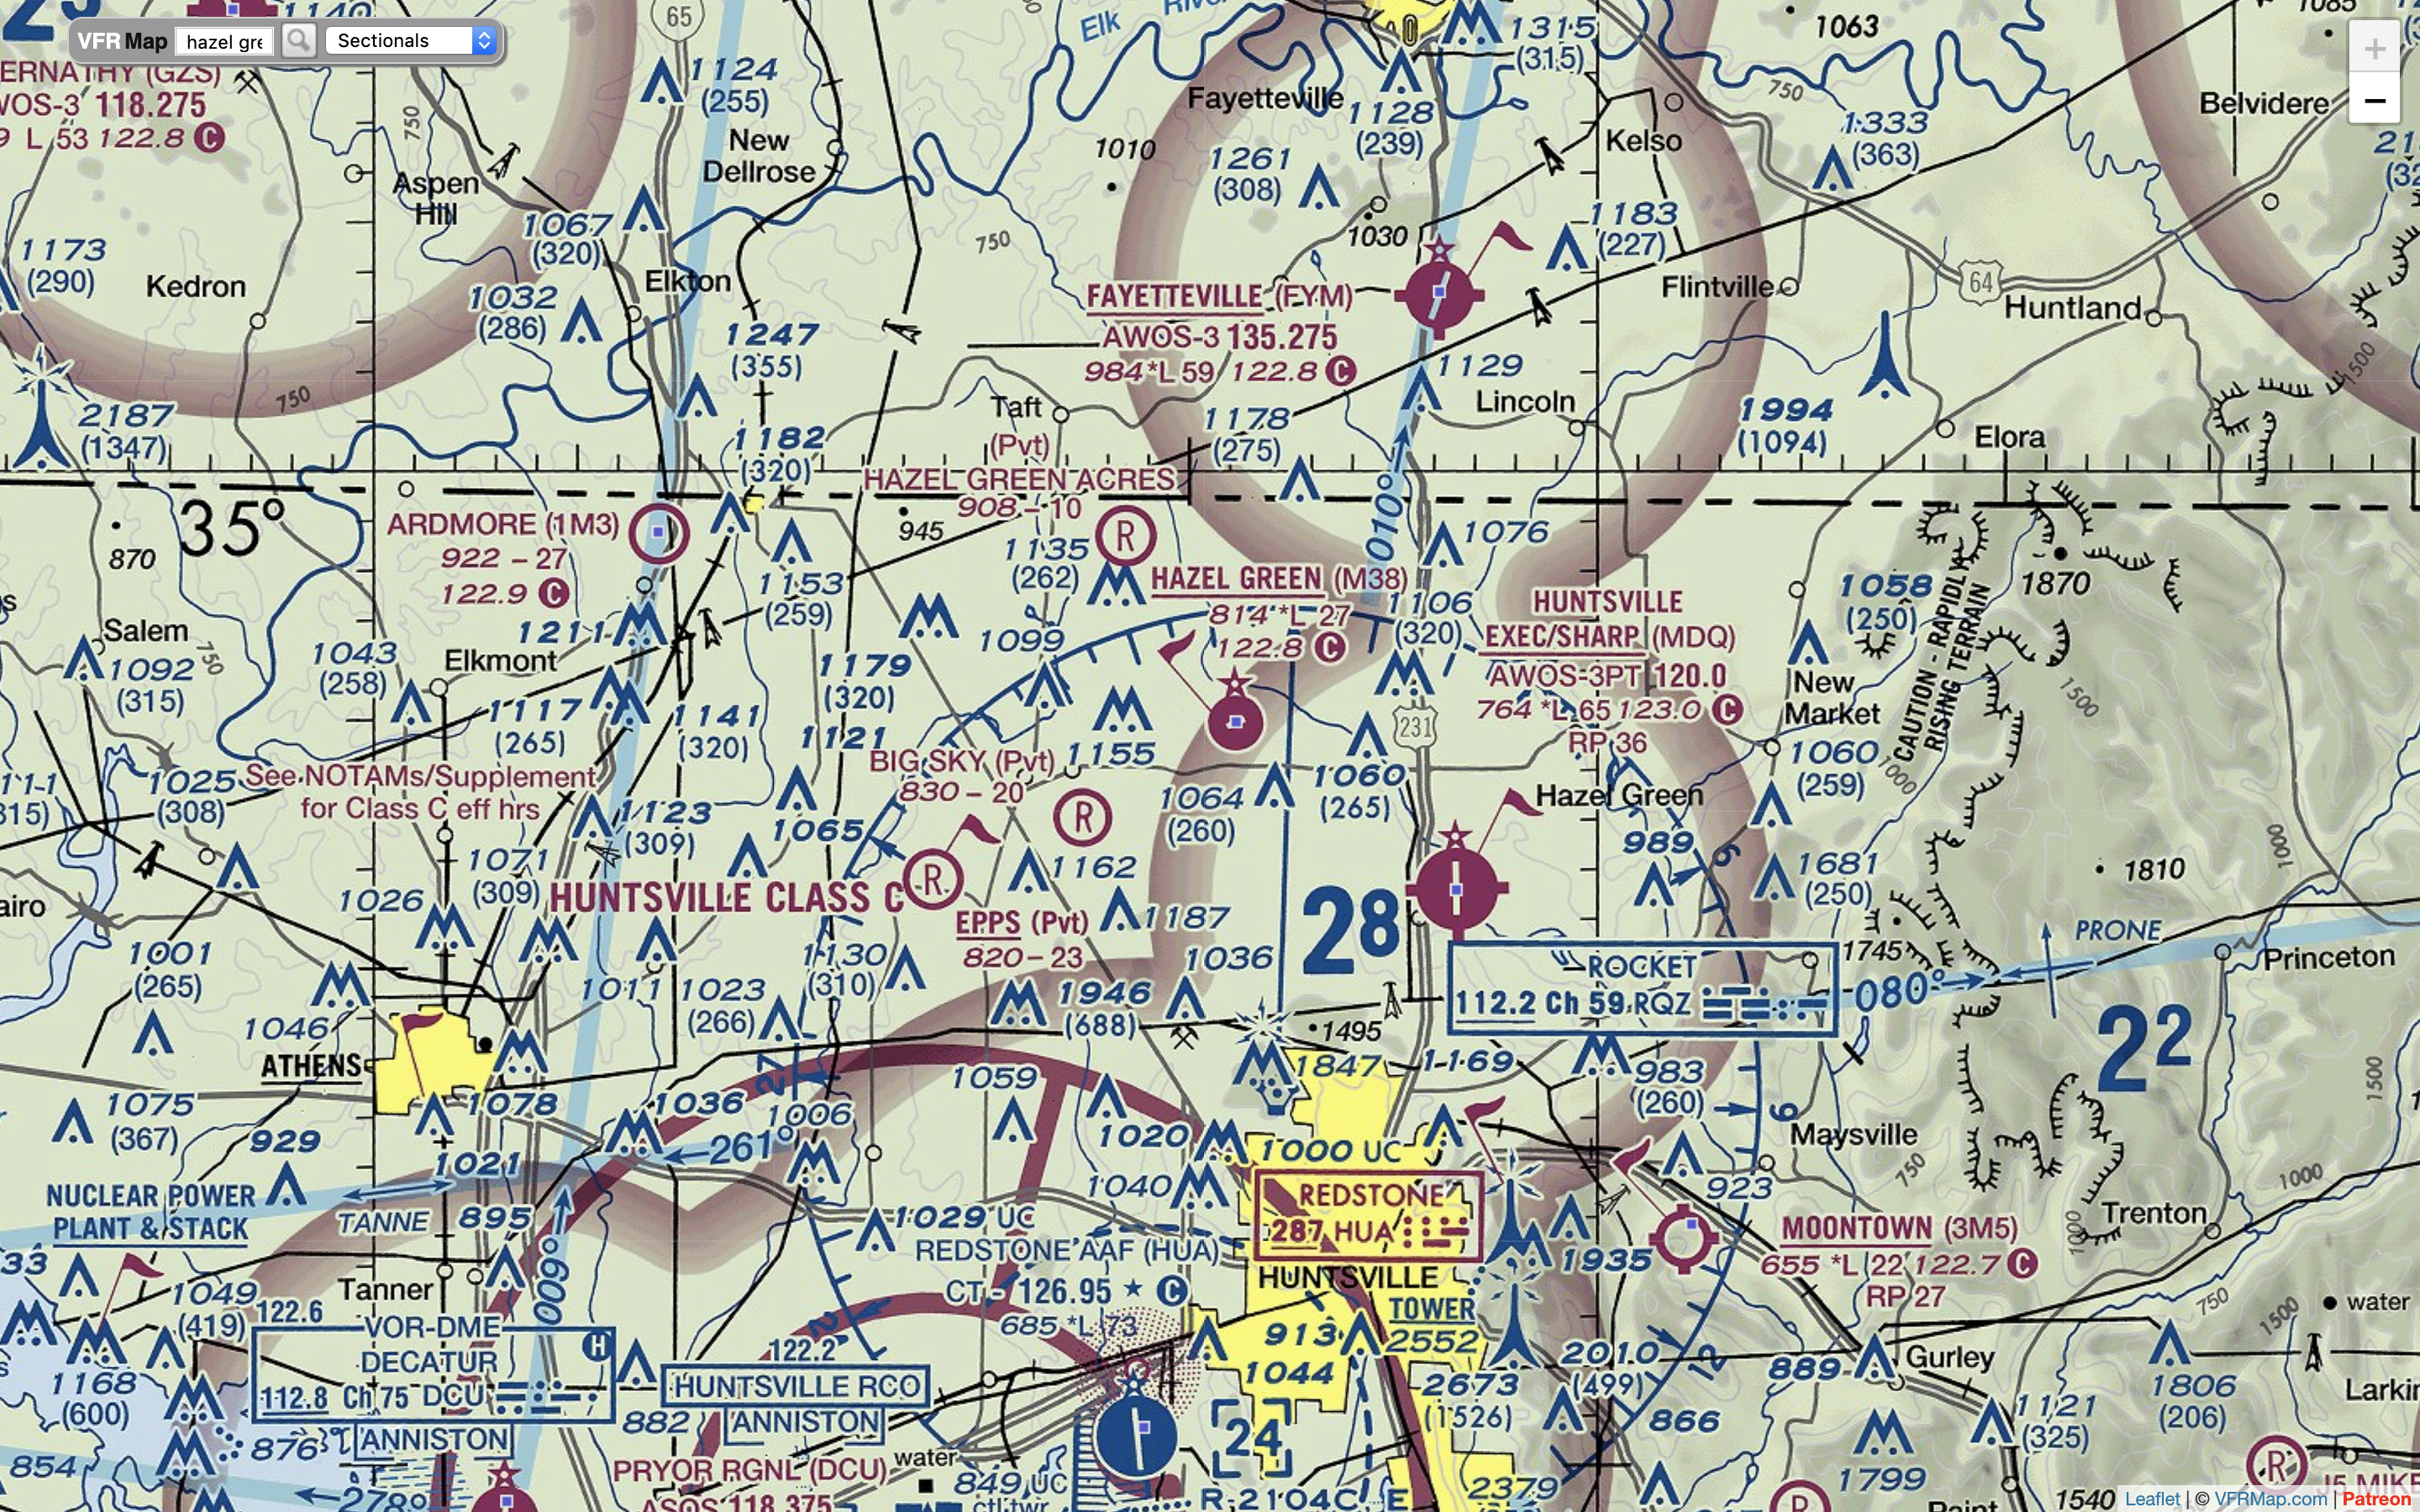
\includegraphics[width=0.75\linewidth]{img/PL/AeronauticalChart}
	\caption[VFR aeronautical chart of the Hazel Green, AL area]{\gls{vfr} aeronautical chart of the Hazel Green, AL area. Adapted from \href{http://vfrmap.com/}{VFRMap.com}}
	\label{fig:PL:Deployment:VFRchart}
\end{figure}

In this chart, the Class E airspace is bounded by a vignette magenta border, and spans down to \SI{700}{\feet}; anything below that is Class G airspace, and thus open for \gls{uav} operations. Incidentally, the area of payload operations lies beyond a 5 mile radius of the closest airfield.

\subsection{Team-derived requirements}

In addition to the above, a number of additional requirements have been compiled by the team. In particular, the robustness of the securement system, as well as the reliability of the deployment system are at the center of the discussion\todo[author=HE]{Draft team-derived requirements}.

\begin{enumerate}[noitemsep, label=\arabic*.]
	\item Deployment
	\begin{enumerate}[noitemsep, label=1.\arabic*.]
		\item UAV Transport 
		\begin{enumerate}[noitemsep, label=1.1.\arabic*.]
			\item The UAV must be securely transported from launch until deployment. There must be no physical damage to the UAV, and its functionality must be maintained.
			\item The security mechanism of the UAV and the UAV itself must be built to be able to withstand FILLER Gs. 
			\item This security mechanism must be released when the rocket reaches 120m as regulated by the FAA. 
		\end{enumerate}
		\item Nose Cone Release
		\begin{enumerate}[noitemsep, label=1.2.\arabic*.]
			\item The nose cone must be safely jettisoned to allow for proper UAV deployment. A safe jettison requires the nose cone's kinetic energy to be less than 100J as it impacts the ground.
			\item A parachute with an area of FILLER must deploy from its stored location in the tip of the nose cone in order to satisfy the kinetic energy requirement as shown in equation FILLER.
		\end{enumerate}
		\item UAV Release
		\begin{enumerate}[noitemsep, label=1.3.\arabic*.]
			\item The UAV must be safely lowered from the payload bay so that it can begin its independent flight.
			\item The lowering mechanism must be able to withstand a force greater than the weight of the UAV.
			\item The lowering mechanism must be able to deploy the UAV within ten seconds of the jettison of the nose cone.
		\end{enumerate}
		\item Critical Systems Check
		\begin{enumerate}[noitemsep, label=1.4.\arabic*.]
			\item A critical systems check must be performed quickly to ensure the UAV's ability to fly independently.
			\item The arms of the UAV must be properly deployed.
			\item The power system of the UAV must functional.
			\item The motors with propellers must be actively running.
			\item The orientation of the UAV must be upright as confirmed by accurate readings from the appropriate sensors.
		\end{enumerate}
		\item Separation Protocol
		\begin{enumerate}[noitemsep, label=1.5.\arabic*.]
			\item There must be a mechanism to detach the UAV from the upper body tube so that it can achieve independent flight.
			\item An automatic maneuver must be executed by the UAV to move itself away from the falling body tube.
		\end{enumerate}
	\end{enumerate}
	\item Hover
	\begin{enumerate}[noitemsep, label=2.\arabic*.]
		\item Take longer Kenneth
		\item \begin{enumerate}[noitemsep, label=2.1.\arabic*.]
			\item For real
		\end{enumerate}
	\end{enumerate}
	\item Landing Protocol
	\begin{enumerate}[noitemsep, label=3.\arabic*.]
		\item Computer Vision Check
		\begin{enumerate}[noitemsep, label=3.1.\arabic*.]
			\item The computer vision program must be working as designed as the UAV approaches GPS waypoint for the landing site of the sample material. The pilot will have to manually confirm that the system is functioning properly.
		\end{enumerate}
		\item IRMA System Check
		\begin{enumerate}[noitemsep, label=3.2.\arabic*.]
			\item The IRMA system must confirm its functionality post-deployment.
			\item The flight computer must confirm that the members of the IRMA can close to scoop the material. 
		\end{enumerate}
		\item UAV Descent on Target
		\begin{enumerate}[noitemsep, label=3.3.\arabic*.]
			\item The UAV must begin to descend towards the ground as it processes its final systems check.
			\item The descent velocity must be kept under FILLER m/s to ensure that any impact with a landing surface does not harm the UAV.
			\item The computer vision software must guide the UAV towards the sample collection site.
			\item The UAV must land upright atop the sample site with a final velocity of 0 m/s.
		\end{enumerate}
	\end{enumerate}
	\item Sample Retrieval Protocol
	\begin{enumerate}[noitemsep, label=4.\arabic*.]
		\item Engage IRMA
		\begin{enumerate}[noitemsep, label=4.1.\arabic*.]
			\item The IRMA must close its members around a collection of the sample.
			\item The UAV pilot must confirm that a sufficient that the IRMA has retrieved a sufficient amount of the sample.
		\end{enumerate}
		\item Return to Hover
		\begin{enumerate}[noitemsep, label=4.2.\arabic*.]
			\item The UAV must return to the altitude of the initial hover.
			\item The IRMA must maintain a sufficient amount of sample.
		\end{enumerate}
		\item Flee Sample Site
		\begin{enumerate}[noitemsep, label=4.3.\arabic*.]
			\item The UAV must move 5m in any cardinal direction from its location above the sample site.
		\end{enumerate}
	\end{enumerate}
\end{enumerate}

\section{Means of Securement}\label{PL:Deployment:Securement}
	\subsection{Locking Mechanism}
		This is a filler paragraph
		
	\subsection{UAV Arm Configuration}
		\subsubsection{Parallel Unfolding Arms}
			This is a filler paragraph

		\subsubsection{Vertically Unfolding Arms}
			This is a filler paragraph

\section{Means of Deployment}\label{PL:Deployment:Deployment}
	\subsection{UAV Release Mechanism}
		\subsubsection{Launch Rails}
			This is a filler paragraph

		\subsubsection{Lowering Mechanism}
			This is a filler paragraph

	\subsection{Nose Cone Jettison}
		\subsubsection{Without Parachute}
			This is a filler paragraph
		
		\subsubsection{With Parachute}
			This is a filler paragraph

\section{Payload Structures}\label{PL:Deployment:Structures}
	\subsection{Landing Leg Design}
		\subsubsection{Retractable Landing Mechanism}
			This is a filler paragraph

		\subsubsection{Static Landing Mechanism}
			This is a filler paragraph

	\subsection{Ice Retrieval and Mobility Agent}
		\subsubsection{Pin Joint Mechanism}
			This is a filler paragraph

		\subsubsection{Sliding Pin Mechanism}
			This is a filler paragraph

		\subsubsection{Wormgear Mechanism}
			This is a filler paragraph

\section{Payload Avionics}\label{PL:Deployment:Avionics}
	\subsection{Computer Vision}
		\subsubsection{Algorithmic Approach}
			This is a filler paragraph

		\subsubsection{Deep Learning Approach}
			This is a filler paragraph

	\subsection{Flight Controller}
		\subsubsection{ArduPilot}
			This is a filler paragraph

		\subsubsection{Pixhawk}
			This is a filler paragraph

		\subsubsection{Navio2}
			This is a filler paragraph

\section{Leading Design}\label{PL:Deployment:LeadingDesign}
	\subsection{Drone Structures}
		\subsubsection{Arm Configuration}
			This is a filler paragraph

		\subsubsection{Landing Legs}
			This is a filler paragraph
	
		\subsubsection{Ice Recovery and Mobility Agent}
			This is a filler paragraph

	\subsection{Avionics}
		\subsubsection{Flight Controller}
			This is a filler paragraph

		\subsubsection{Computer Vision}
			This is a filler paragraph

\section{Testing Campaign}\label{PL:Deployment:Testing}
	\subsection{Structual Testing}
		\subsubsection{Deployment Tests}
			This is a filler paragraph

		\subsubsection{Ice Retrieval and Mobility Agent Tests}
			This is a filler paragraph

	\subsection{Avionics Testings}
		\subsubsection{Flight Controller Tests}
			This is a filler paragraph

		\subsubsection{Computer Vision Tests}
			This is a filler paragraph





